\part{Server}
\label{server}

Server sdružuje všechny klienty, kteří se na něj připojí a umožnuje případnou vzájemnou komunikaci. Server může po připojení vyžadovat autentikaci uživatele pomocí jména a hesla.

\chapter{Client}

Každý připojený fyzický klient má na serveru svou virtuální reprezentaci. Je reprezentován pomocí unikátního ID v rozmezí $0$ až $2^{32} - 1$ a svého uživatelského jména. Uživatelské jméno může být na serveru dupliciní, záleží na implementaci serveru, jestli tuto možnost spřístupnuje.

\chapter{Rooms}

Na serveru se nacházejí místnosti, v rámci nichž mezi sebou uživatelé komunikují. Na serveru nemusí být žádná a nebo až $2^{32}$ místností (4 bytové ID). Místnosti mají své ID a jméno. Místnost může být otevřená všem, nebo zamčená heslem.

Klienti spolu na serveru mohou komunikovat jen v případě, že se naházejí ve stejné místnosti. Každý klient se po připojení nenachází v žádné místnosti, do té se však může následně připojit. Klient se může do místností připojovat jen v případě, že se nenachází v žádné jiné. Logický důsledek je, že se klient může nacházet jen v jedné místnosti v jeden okamžik. Klienti se mohou do místností připojovat, odpojovat a místnosti vytvářet. V případě, že klient vytvoří novou místnost je do ní automaticky připojen. Místnost existuje jen po dobu co se v ní nachází alespon jeden klient, prázdné místnosti jsou automaticky mazány. Místnosti na serveru ilustruje obrázek \ref{server.pictures.server_client_rooms}.

\begin{figure}[h]
  \centering
  \includegraphics[width=0.80\textwidth]{diagrams/server_client_rooms.png}
  \caption{Clients, server and rooms}
  \label{server.pictures.server_client_rooms}
\end{figure}

\section{Canvases and layers}

Hlavním cílem protokolu je umožnit uživatlům sdílené kreslení. To je zajištováno v rámci místností pomocí jednotlivých plánek a vrstev. V rámci místnosti může existovat několik pláten (samostatných obrázků) v nichž jsou vrstvy (které se překrývají) do nichž klienti kreslí. Strukturu místnosti ilustruje obrázek \ref{server.pictures.room}.

\begin{figure}[h]
  \centering
  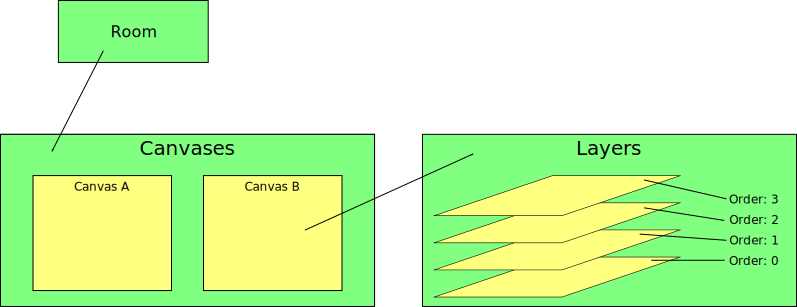
\includegraphics[width=0.80\textwidth]{diagrams/room.png}
  \caption{Room}
  \label{server.pictures.room}
\end{figure}

Všechny plátna mají své rozměry (v pixelech), jméno a ID. Server se nestará o pořadí pláten, je plně na klientovy jakým způsobem je zobrazuje. Dále obsahují vrstvy a poskytují jejich pořadí.

Každá místnost může obsahovat $0$ až $2^{32}$ (4 bytové ID) pláten a každé plátno se skládá z z $0$ až $2^{32}$ vrstev.

Plátno má své ID, pořadí a vlastní obsah (obrázek s $32$ bitovou hloubkou -- 1\,{}B je vyhrazen jako alpha channel).

Pořadí vrstev začíná číslem $0$ a končí $p - 1$, kde $p$ je celkový počet vrstev. Při vykreslování se nejvíce dospod (takže jako první) kreslí vrstva s pořadím $0$. Takže čím větší má vrstva pořadí, tím více navrchu je vykreslena. Viz obrázek \ref{server.pictures.room}.

\section{Chat}

\section{Another services}


